\documentclass[12pt]{report} 

% PACKAGES 
\usepackage[dutch]{babel}
\usepackage[utf8]{inputenc}
\usepackage{color}
\usepackage{amsmath} % Matrices
\usepackage{empheq}
\usepackage{booktabs}
\usepackage{xcolor}
\usepackage{sectsty}
\usepackage{lipsum}
\usepackage{enumitem}
\usepackage{pgfplots}
\pgfplotsset{compat=1.13}



\partfont{\color{brown}}
\chapterfont{\color{teal}}
\sectionfont{\color{cyan}}

% DOCUMENT INFORMATION
\title{Fysica: mechanica, optica en moderne fysica}
\author{Bert De Saffel}
\date{2017-2018}


% CUSTOM COMMANDS
\newcommand{\todo}[1] {
\color{red}\textunderscore{\textit{TODO: #1}}
}

\newcommand{\important}[1] {\textbf{\color{orange}#1}}

% DOCUMENT
\begin{document}
\maketitle
\tableofcontents

\chapter{Foutentheorie}
\section{Testvragen}
De oefeningen op Curios zijn analoog aan de test
\begin{enumerate}
 \item Foute notatie omvormen naar juiste notatie.
 \item Complete foute notatie. De eenheid en macht van 10 moet helemaal achteraan staan. De meetfout 
 moet 1 of 2 beduidende cijfers bedragen en het waardegetal moet even nauwkeurig zijn als de meetfout.
 \item Meetfoutberekening (Combinatie van som, verschil, product, deling, macht, sin en cos).
 \item Fout op gemiddelde. Je moet de standaarddeviatie kunnen uitrekenen van gegeven data.
 \item Grafiekanalyse. Neem de formule, vorm deze om naar $y = ax + b$. Kijk in uw formule wat
 overeenkomt met a en b.
\end{enumerate}

\section{Vorm}
\important{Gemeten waarde} $\pm$ \important{absolute fout(AF)}
\begin{itemize}
 \item 6,458 $\pm$ 0,027 mV
 \item 8,67  $\pm$ 0.05 . 10$^3$m
\end{itemize}
\important{Relative Fout(RF)} = $\frac{AF}{Gemeten\;waarde}$
\begin{itemize}
 \item RF = $\frac{0,027}{6,458} = 0.04 = 0.4\%$
 \item RF = $\frac{0,05\;.\;10^3}{8,67} = 5.77 = 577\%$
\end{itemize}
\section{Soorten}
\begin{enumerate}
 \item Fout op meting
 \item Statistische fout
 \item Fout op berekening
\end{enumerate}

\subsection{Fout op meting}
\begin{itemize}
 \item Is afhankelijk van de nauwkeurigheid van het meettoestel
 \item Op een meetlat: $\pm 1mm$
 \item Op een chronometer: $\pm 0.01s$
\end{itemize}
Meten van de lengte van een tafel met een meetlat: $5 \pm 1.10^{-3} m$ 

\subsection{Statistische fout}

Dezelfde lengten van een tafel 5 keer meten met een meetlat = 
Het gemiddelde nemen van de gemeten waarden en het gemiddelde van de absolute
fouten

Voorbeeld: We meten de slingerperiode met een chronometer tot op 0.01s nauwkeurig een 
aantal keer. De resultaten zijn 3.29s; 3.12s; 3.45s; 3.18s; 3.21s; 3.26s.
Wat is de gemiddelde periode?
\begin{enumerate}
 \item Gemiddelde = 3,25
 \item standaarddeviatie = 0,114
 \item Fout op gemiddelde = $\frac{stdev}{\sqrt{6}}$ = 0,05
 \item Resultaat = $3,25 \pm 0,05 s$
\end{enumerate}


\subsubsection{Grafiekanalyse}
$$ \frac{V}{V_{max}} = \frac{S}{K_m + S} $$
\begin{tikzpicture}
 \begin{axis}[ ticks=none,
      xlabel = {$S^{-1} (\frac{dm^{3}}{mol})$},
      xticklabels = {,,},
      axis x line = bottom,
      xmin = 0, xmax = 1,
      ylabel = {$V^{-1} [\frac{sg}{mol}]$},		
      ylabel style = {rotate=-90},
      yticklabels = {,,},
      axis y line = left,
      ymin = 0, ymax = 1,
    ]
 \end{axis}
 \draw (0,0) -- (5,5);
 \node at (1, 1.1) {\textbullet};
 \node at (2.2, 1.9) {\textbullet};
 \node at (2.7, 2.9) {\textbullet};
 \node at (3.5, 3.5) {\textbullet};
 \node at (4.3, 3.7) {\textbullet};
 \node[draw, text] at (6,3) {y = 0.468x + 3.55};

\end{tikzpicture}
\\
$ y = ax + b $
\\
$a: (\frac{sg}{mol})/(\frac{dm^{3}}{mol}) = \frac{sg}{dm^3}$
\\
$b: \frac{sg}{mol} $
\\
$$v^{-1} = \frac{K_m}{V_{max}}S^{-1} + \frac{1}{V_{max}}$$

\subsection{Fout op berekening}
Voor de voorbeelden worden volgende X en Y gebruikt: \newline
$X = 16,5 \pm 0.5 $
\newline
$Y = 237,1 \pm 0.9 $
\begin{itemize}
 \item \important{Som/Verschil}: $AF(R) = \sqrt{AF(X)^2 + AF(Y)^2}$
 \begin{enumerate}
  \item $X + Y = ?$
  \item $AF(R) = \sqrt{0,5^2 + 0,9^2}$
  \item $AF(R) = \sqrt{1,06}$
  \item $AF(R) = 1,03$
  \item $16,5 + 237,1 \pm 1,03$
  \item \important{$253,6 \pm 1,0$}
 \end{enumerate}
 \begin{enumerate}
  \item $X - Y = ?$
  \item $AF(R)_{X-Y} = AF(R)_{X+Y}$ 
  \item \important{$220,6 \pm 1,0$}
 \end{enumerate}
 \item \important{Product/Deling}: $RF(R) = \sqrt{RF(X)^2 + (RF(Y)^2}$
  \begin{enumerate}
   \item $X * Y = ?$
   \item $RF(R) = \sqrt{(\frac{0,5}{16,5})^2 + (\frac{0,9}{237,1})^2}$
   \item $RF(R) = 0,03$
   \item $16,5 * 237,1 = 3912,15$
   \item $AF(R) = 3912,15 * RF(R)$
   \item $AF(R) = 3912,15 * 0,03$
   \item $AF(R) = 117,38$
   \item \important{$3912,2 \pm 117,4$}
  \end{enumerate}
  \begin{enumerate}
   \item $\frac{X}{Y} = ?$
   \item $RF(R)_{\frac{X}{Y}} = RF(R)_{X * Y}$
   \item $RF(R) = 0,03$
   \item $\frac{16,5}{237,1} = 0,0696$
   \item $AF(R) = 0,0696 * 0.03$
   \item $AF(R) = 0,0021$
   \item \important{$0,0696 \pm 0,0021$}
  \end{enumerate}
  \item {\important{Macht/Wortel}: $RF(R) = nRF(X)$}
  \begin{enumerate}
   \item $x^3 = ?$
   \item $RF(R) = 3RF(X)$
   \item $RF(R) = 0,09$
   \item $(16,5)^3 \pm 0,09$
   \item \important{$4492,13 \pm 0,09$}
  \end{enumerate}
  \begin{enumerate}
   \item $\sqrt[3]{x} = ?$ 
   \item $x^{\frac{1}{3}}$
   \item $RF(R) = \frac{1}{3}RF(X)$
   \item $RF(R)  = 0,1$
   \item $\sqrt[3]{16,5} \pm 0,1$
   \item \important{$2,5 \pm 0,1$}
  \end{enumerate}
  
  \item{\important{Functies}}
  \begin{enumerate}
   \item $tg(45\;45' \pm 3') = ?$
   \item $3' = \frac{3}{60} graden = \frac{\pi}{3600}rad$
   \item $AF(tg(X)) = \frac{1}{cos^2x}.AF(X)$
   \item $AF(tg(X)) = \frac{1}{cos^2x}*\frac{\pi}{3600}$
   \item $AF(tg(X)) = 0,0018$
   \item $tg(45\;45') \pm 0,0018$
   \item \important{$1,0265 \pm 0,0018$}
  \end{enumerate}



\end{itemize}




\part{Mechanica}
\chapter{Beweging in 2 en 3 dimensies}
\section{Algemeen}

$$\overrightarrow{v}_{tot} = \overrightarrow{v}_1 + \overrightarrow{v}_2 + ... + \overrightarrow{v}_n$$

$$
 \begin{cases}
  \overrightarrow{v} = \frac{d\overrightarrow{r}}{dt} \\
  \overrightarrow{a} = \frac{d\overrightarrow{v}}{dt}
 \end{cases}
$$

$$
 \begin{cases}
  \overrightarrow{v}_{gem} = \frac{\Delta\overrightarrow{r}}{\Delta t} \\
  \overrightarrow{a}_{gem} = \frac{\Delta\overrightarrow{v}}{\Delta t}
 \end{cases}
$$

\section{Eenparige beweging (constante versnelling)}

$$
 \begin{cases}
  \overrightarrow{r} = \overrightarrow{r}_0 + v_0t + \frac{at^{2}}{2} \\
  \overrightarrow{v} = \overrightarrow{v}_0 + at
 \end{cases}
$$

$$
 \begin{cases}
  x = x_0 + v_{0x}t + \frac{a_xt^{2}}{2} \\
  v_x = v_{0x} + a_xt
 \end{cases}
$$

$$
 \begin{cases}
  y = y_0 + v_{0y}t + \frac{a_yt^{2}}{2} \\
  v_y = v_{0y} + a_yt
 \end{cases}
$$



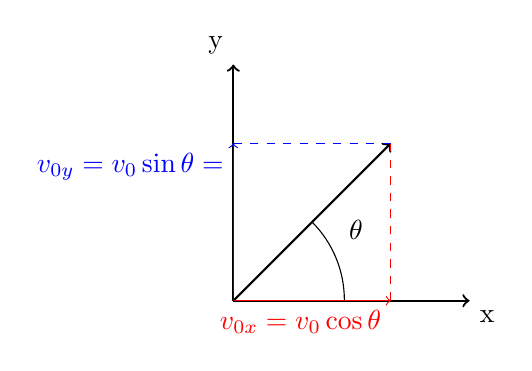
\begin{tikzpicture}

\coordinate (O) at (0,0);
\coordinate (A) at (2,2);
\coordinate (X) at (2,0);
\coordinate (Y) at (0,2);

\draw[thick, ->] (O) -- (3, 0) node[anchor=north west] {x};
\draw[thick, ->] (O) -- (0, 3) node[anchor=south east] {y};
\draw[thick, ->] (O) -- (A);
\draw[red, ->] (O) -- (X) node[anchor = north east] {$v_{0x} = v_0\cos\theta$};
\draw[blue, ->] (O) -- (Y) node[anchor = north east]{$v_{0y} = v_0\sin\theta = $};
\draw[red, dashed] (X) -- (A);
\draw[blue, dashed] (Y) -- (A);

\draw (1,1) arc(45:0:1.4);
\node[] at (30:1.8) {$\theta$};
\end{tikzpicture}


\section{Eenparige cirkelbeweging}
$a = \frac{v^{2}}{r}$

\begin{tikzpicture}
 \draw (0,0) circle (3cm);
 
 \draw (0, 0) -- (2.12, 2.12) node[anchor=south] {$r$};
 
 
 \draw[thick, ->, red] (0, -3) -- (0, -2)  node[anchor=east] {$\overrightarrow{a}$};
 \draw[thick, ->, blue] (0, -3) -- (1 , -3) node[anchor=north] {$\overrightarrow{v}$};
 
 \draw[thick, ->, red] (3, 0) -- (2, 0) node[anchor=north east] {$\overrightarrow{a}$};
 \draw[thick, ->, blue] (3, 0) -- (3 , 1) node[anchor=west] {$\overrightarrow{v}$};

 \draw[thick, ->, red] (0, 3) -- (0, 2) node[anchor=east] {$\overrightarrow{a}$};
 \draw[thick, ->, blue] (0, 3) -- (-1 ,3) node[anchor=south] {$\overrightarrow{v}$};
 
 \draw[thick, ->, red] (-3, 0) -- (-2, 0) node[anchor=west] {$\overrightarrow{a}$};
 \draw[thick, ->, blue] (-3, -0) -- (-3 , -1) node[anchor=east] {$\overrightarrow{v}$};
 
 \node at (0, 0) {\textbullet};
\end{tikzpicture}





\chapter{Kracht en beweging}
\section{Begrippen}
\begin{itemize}
\item {\important{Eerste wet van Newton}: Een voorwerp in uniforme beweging blijft in uniforme beweging. Een voorwerp in 
rust blijft in rust.}
\item {\important{Tweede wet van Newton}: De verandering in snelheid is gelijk aan de netto kracht die uitgeoefend wordt op het voorwerp}
\item {\important{Derde wet van Newton}: Als voorwerp A een kracht uitoefend op voorwerp B, dan zal B een tegengestelde kracht uitoefenen op A}

\end{itemize}

\section{Formules}
\begin{itemize}
  \item {\important{Tweede wet van Newton}: 
  $\underline{\overrightarrow{F}_{net} = m\overrightarrow{a}}$ met $\overrightarrow{F}_{net}$ de som van de vectoren van alle krachten die worden uitgeoefend 
  op het voorwerp, en $ma$ het product van de massa van het voorwerp en zijn versnelling.}
  \item {\important{Gewicht}: $\underline{\overrightarrow{w} = m\overrightarrow{g}}$ met $m$ de massa van het voorwerp en $g$ de gravitatieconstante}
  \item {\important{Wet van Hooke (veren)}: $\underline{F_{s} = -kx}$ met $k$ de krachtconstante van de veer en $x$ de afstand}
  \item {\important{Lineair momentum}: 
  $\underline{\overrightarrow{p} = m\overrightarrow{v}}$ 
  met $\overrightarrow{p}$ de impuls, $m$ de massa en $\overrightarrow{v}$ de snelheid.
  }
\end{itemize}

\section{Vraagstukken met wetten van Newton}

\chapter{Toepassen wetten van Newton}
\section{Algemeen}
$$\sum \overrightarrow{F} = m\overrightarrow{a} \Rightarrow 
\begin{cases}
  \sum \overrightarrow{F}_x = m\overrightarrow{a_x} \\
  \sum \overrightarrow{F}_y = m\overrightarrow{a_y} 
 \end{cases}
$$
Bij elk vraagstuk zeker kijken naar:
\begin{itemize}
 \item Zwaartekracht
 \item Normaalkracht
 \item Wrijvingskracht
\end{itemize}


\section{Wrijving}
$$ F_{w} = \mu N$$
Zolang $F_w \leq \mu N$ dan spreken  we over statische wrijving, anders spreken we over kinetische wrijving.
\section{Veerkracht}
$$ F_v = -kx $$


\chapter{Arbeid, energie en vermogen}
\section{Arbeid}
$$ W = \int_{\overrightarrow{r}_1}^{\overrightarrow{r}_2} \overrightarrow{F} \; d\overrightarrow{r}$$
Bovenstaande formule zegt hoeveel energie er nodig.
$$\Rightarrow W = F_{||} \Delta\overrightarrow{r}$$
De componenten evenwijdig met de as leveren arbeid
\section{Vermogen}
$$ P = \frac{dw}{dt} \Rightarrow 
\begin{cases}
   P = \overrightarrow{F}\overrightarrow{v} \;\;\;\;\;\; (ogenblikkelijk) \\ 
   P = \frac{\Delta w}{\Delta t} \;\;\;\;\;\;\;\; (periode)
\end{cases}
$$
\chapter{Behoud van energie}
\section{Algemeen}
$$K_0 + U_0 + W_{nc} = K_1 + U_1$$
Conservatieve energie : Energie dat je terugkrijgt
\begin{itemize}
 \item zwaartekracht
 \item veer
\end{itemize}
Niet coneservative energie : Energie dat verloren is
\begin{itemize}
 \item wrijving
 \item duwkracht
 \item trekkracht
\end{itemize}

$$ K = \frac{mv^{2}}{2}$$
$$ U \Rightarrow 
\begin{cases}
  mgh \;\;\;\;\;\; (zwaartekracht)\\ 
  \frac{kx^{2}}{2} \;\;\;\;\;\;\;\; (veer)
\end{cases}
$$



\chapter{Systemen van deeltjes}
\section{Impuls}
$$\overrightarrow{p} = m\overrightarrow{v}$$
$$\sum \overrightarrow{p}_v = \sum \overrightarrow{p}_n$$
\begin{itemize}
 \item Bij een elastische botsing: $\sum \overrightarrow{K}_v = \sum \overrightarrow{K}_n$ 
 \item Bij een niet elastische botsing: /
 \item Bij een volkomen onelastische botsing: Alle voorwerpen hangen na de botsing aan elkaar en 
 bewegen voort als één voorwerp. Hieruit volgt $m_n = \sum_i m_i$
 \item Bij een 1 dimensionale elastische botsing: $v_{1v} - v_{2v} = -(v_{1n} - v_{2n})$
\end{itemize}

\chapter{Rotatiebewegingen}
\section{Traagheidsmoment}
$$ I_O = I_C + md^2$$
\section{Krachtmoment}
$$\overrightarrow{\tau} = \overrightarrow{r}\overrightarrow{F}$$
$$
\begin{tikzpicture}
 \coordinate (O) at (0,0);
 \coordinate (A) at (2,0);
 \coordinate (B) at (4,2);
 \coordinate (C) at (4,0);
 
 \draw[red, thick, ->] (O) -- (A) node[anchor=north east] {$\overrightarrow{r}$};
 \draw[blue, thick, ->] (A) -- (B) node[anchor= west] {$\overrightarrow{F}$};
 
 \draw[dashed, cyan] (B) -- (C) node[anchor=south west] {$F_\perp$};
 \draw[dashed] (A) -- (C);

\end{tikzpicture}
$$

$$|\overrightarrow{\tau}| = rF_\perp$$
\section{Conversies}
\begin{itemize}
 \item $r = \theta$
 \item $v = \omega$
 \item $a = \alpha$
 \item $m = I_O$
 \item $F = \tau$
 \item $p = L$
\end{itemize}
\section{Conversies - Voorbeelden}
\begin{itemize}
 \item $\overrightarrow{r} = \overrightarrow{r}_0 + v_0t + \frac{at^{2}}{2} 
 \\ \Rightarrow \theta = \theta_0 + \omega_0t + \frac{\alpha t^{2}}{2}$
 \item $\sum \overrightarrow{F} = m\overrightarrow{a}
 \\ \Rightarrow \sum \tau = I\alpha$
 \item $K = \frac{mv^{2}}{2}
 \\ \Rightarrow K = \frac{Iw^{2}}{2}$
\end{itemize}




\chapter{Rotatie vektoren en impulsmoment}

\chapter{Statisch evenwicht}

\chapter{Trillingen}

\chapter{Golven}

\chapter{Electromagnetische golven}

\part{Optica}

\chapter{Breking en terugkaatsing}

\chapter{Beelden en optische instrumenten}

\chapter{Interferentie en diffractie}

\chapter{Deeltjes en golven}

\part{Kernfysica}
\chapter{Kernfysica}



\end{document}
